%!TEX root = ../thesis.tex
\section{Automatic Tracking Techniques}
Kinectograph streams the video view captured from a Kinect camera to a PC. This PC also acts as a web server, publishing the control interface to tablet or phone clients. When a user enables automatic tracking, the PC analyzes user movements using the skeletal data from the Kinect SDK. Based on the user position, it sends appropriate commands to the motorized dock via USB to move the camera (Figure~\ref{fig:architecture}).

\subsection{Hardware}
To control the camera view, Kinectograph utilizes the motor system and base provided by the Kubi\footnote{http://www.revolverobotics.com/}, a dynamic telepresence solution for video calls. This connects to the Kinect with a 3D printed holder (Figure~\ref{fig:figure1}). The Kubi uses two Dynamixel AX-12 motors\footnote{http://www.crustcrawler.com/motors/AX12/index.php}, to pan and tilt. Instead of using Kubi's motor control API and microcontroller, we connect Kubi's motors to an external Arduino Mega (ATmega1280)\footnote{http://arduino.cc/en/Main/arduinoBoardMega} so we can better customize the control of the Dynamixel motors.
% To control the camera view, we designed a specialized dock that holds the Kinect sensor and that can be rotated using a pan-and-tilt servo kit in two axes (Figure~\ref{fig:device}). A bottom servo moves the Kinect left and right (180 degrees), while the top servo moves it up and down (90 degrees from horizon in order to capture the user working area). The mount allows full 180-degree rotation for both horizontal and vertical axis. To control the servo motors of the pan-tilt mechanism, an embedded microcontroller (8-bit ATmega32U4) generates PWM (Pulse-Width Modulation) signals. A base, fabricated on a Projet HD 3000 printer, stabilizes the system and houses the electronics.

%The bottom servo of the pan-tilt system fastens to the middle of the base, while the Kinect holder attaches the Kinect to the pan-tilt system .

% \begin{figure}[t]
% \centering
% 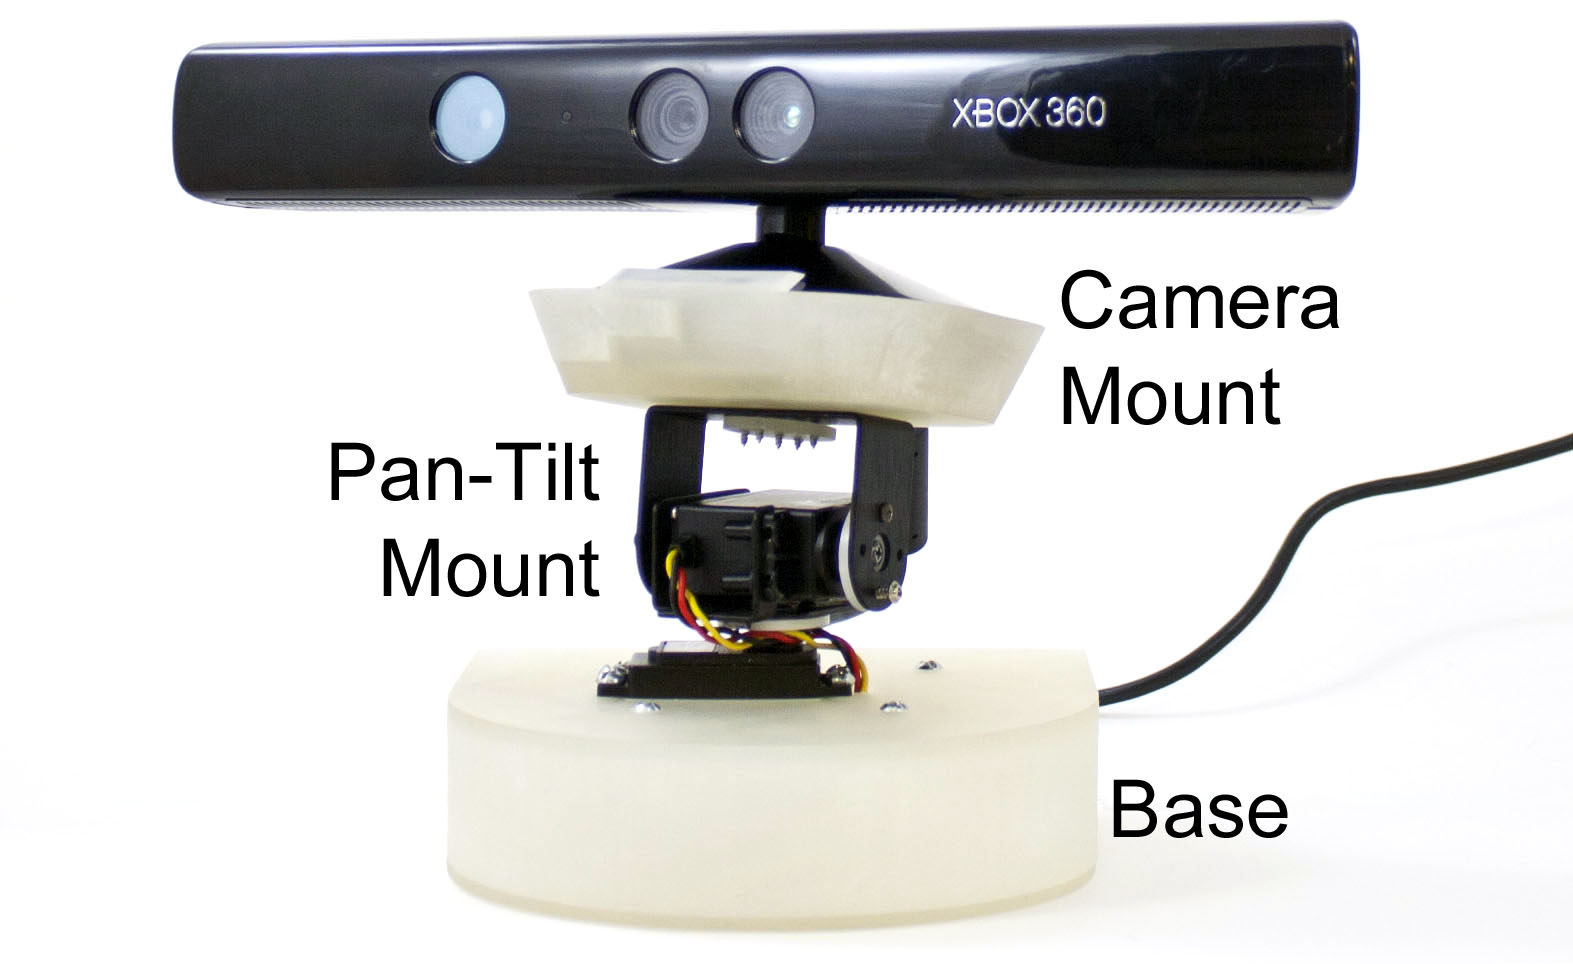
\includegraphics[width=0.7\columnwidth]{device-annotated.jpg}
% \caption{The Kinectograph device combines a depth camera and a robotic pan-tilt mount.}
% \label{fig:device}
% \end{figure}

\subsection{Auto-Tracking Algorithm}

\subsubsection{Motion Tracking and Servo Adjustment}
To track the user position and determine the camera angle, our system analyzes the skeletal tracking data and depth information of a user’s body parts received from the Kinect sensor in real-time. Using Kinect enables the user to freely move or turn around, with support of self-occlusion \cite{Shotton:2011ud}. Currently Kinectograph tracks one or two people. If more people are present, only the two closest are tracked.

\subsubsection{Physical Tracking of Joints}
Kinectograph angles the camera to position the target, such as a user's hand, in the center of the camera view. When a user is found in the view, it receives the position of the tracked joint located at $\textless pos_{x}$, $pos_{y}$, $pos_{z} \textgreater$ in the 3D space that represents a {\em x-y} coordinate and {\em z} as the depth information of the target. The rotation angles are computed in order to align the target joint to the position of the center of view at $\textless center_{x}$, $center_{y}$, $pos_{z}\textgreater$  on the same X-Y plane as the joint position. The rotation angles $\theta_{tilt}$ and $\theta_{pan}$ (in degrees) to tilt or pan the camera are:

Tilt angle of y-axis:
% Θ_tilt=∆y/∆z=arctan⁡((center_y-pos_y)/(pos_z ))
$\theta_{tilt}=\frac{\Delta y}{\Delta z}=\arctan{(\frac{center_{y}-pos_{y}}{pos_{z}})}$

Pan angle of x-axis:
% ∆Θ_pan=∆x/∆z=arctan⁡((center_x-pos_x)/(pos_z ))
$\theta_{pan}=\frac{\Delta x}{\Delta z}=\arctan{(\frac{center_{x}-pos_{x}}{pos_{z}})}$

Figure \ref{fig:math} depicts the geometric relations from the Kinectograph view. Every 10 ms the top motor turns by $\theta_{tilt}$ and the bottom motor turns by $\theta_{pan}$. To avoid extraneous small camera movements, a variable bounding box around the center of the field of view is set such that the Kinectograph only moves once the tracked object leaves the bounding box.

% Our current Kinectograph prototype limits users to selecting only joints in the upper portion of their body. Tracking joints such as the feet may cause the parts of the user to be out of the Kinect camera's view and thus be difficult to recognize. More sophisticated techniques may take into account the distance of the user and the availability of other joints in order to decide when it would be appropriate to track such joints. %For example, allow users to only track the feet, Kinectograph is confident that this would not cause the user to be unrecognizable.

% \subsubsection{Tracking Multiple Joints and Multiple Actors}
To support multiple target selection, we use the same $\theta_{tilt}$ and $\theta_{pan}$ formulas as above, except $\textless pos_{x}$, $pos_{y}$, $pos_{z} \textgreater$ represents the average of all tracked joint positions rather than the position of one tracked joint.
%
% Given...we can move the camera to position multiple targets (i.e. multiple body joints)
If there is more than one actor in the view, users can select joints from the second user. All selected joints are treated equally to be tracked, and thus the camera angle adjustment works as it does in the previous multiple-joint scenario.

%This method was used for Kinectograph's first prototype for simplicity reasons, with knowledge that their would be limitations. We discuss these limitations farther in our Second User Study section.
% add notes about limitations somewhere else down there about wide anglea nd
% smarter tracking physical limitation

\begin{figure}[t]
\centering
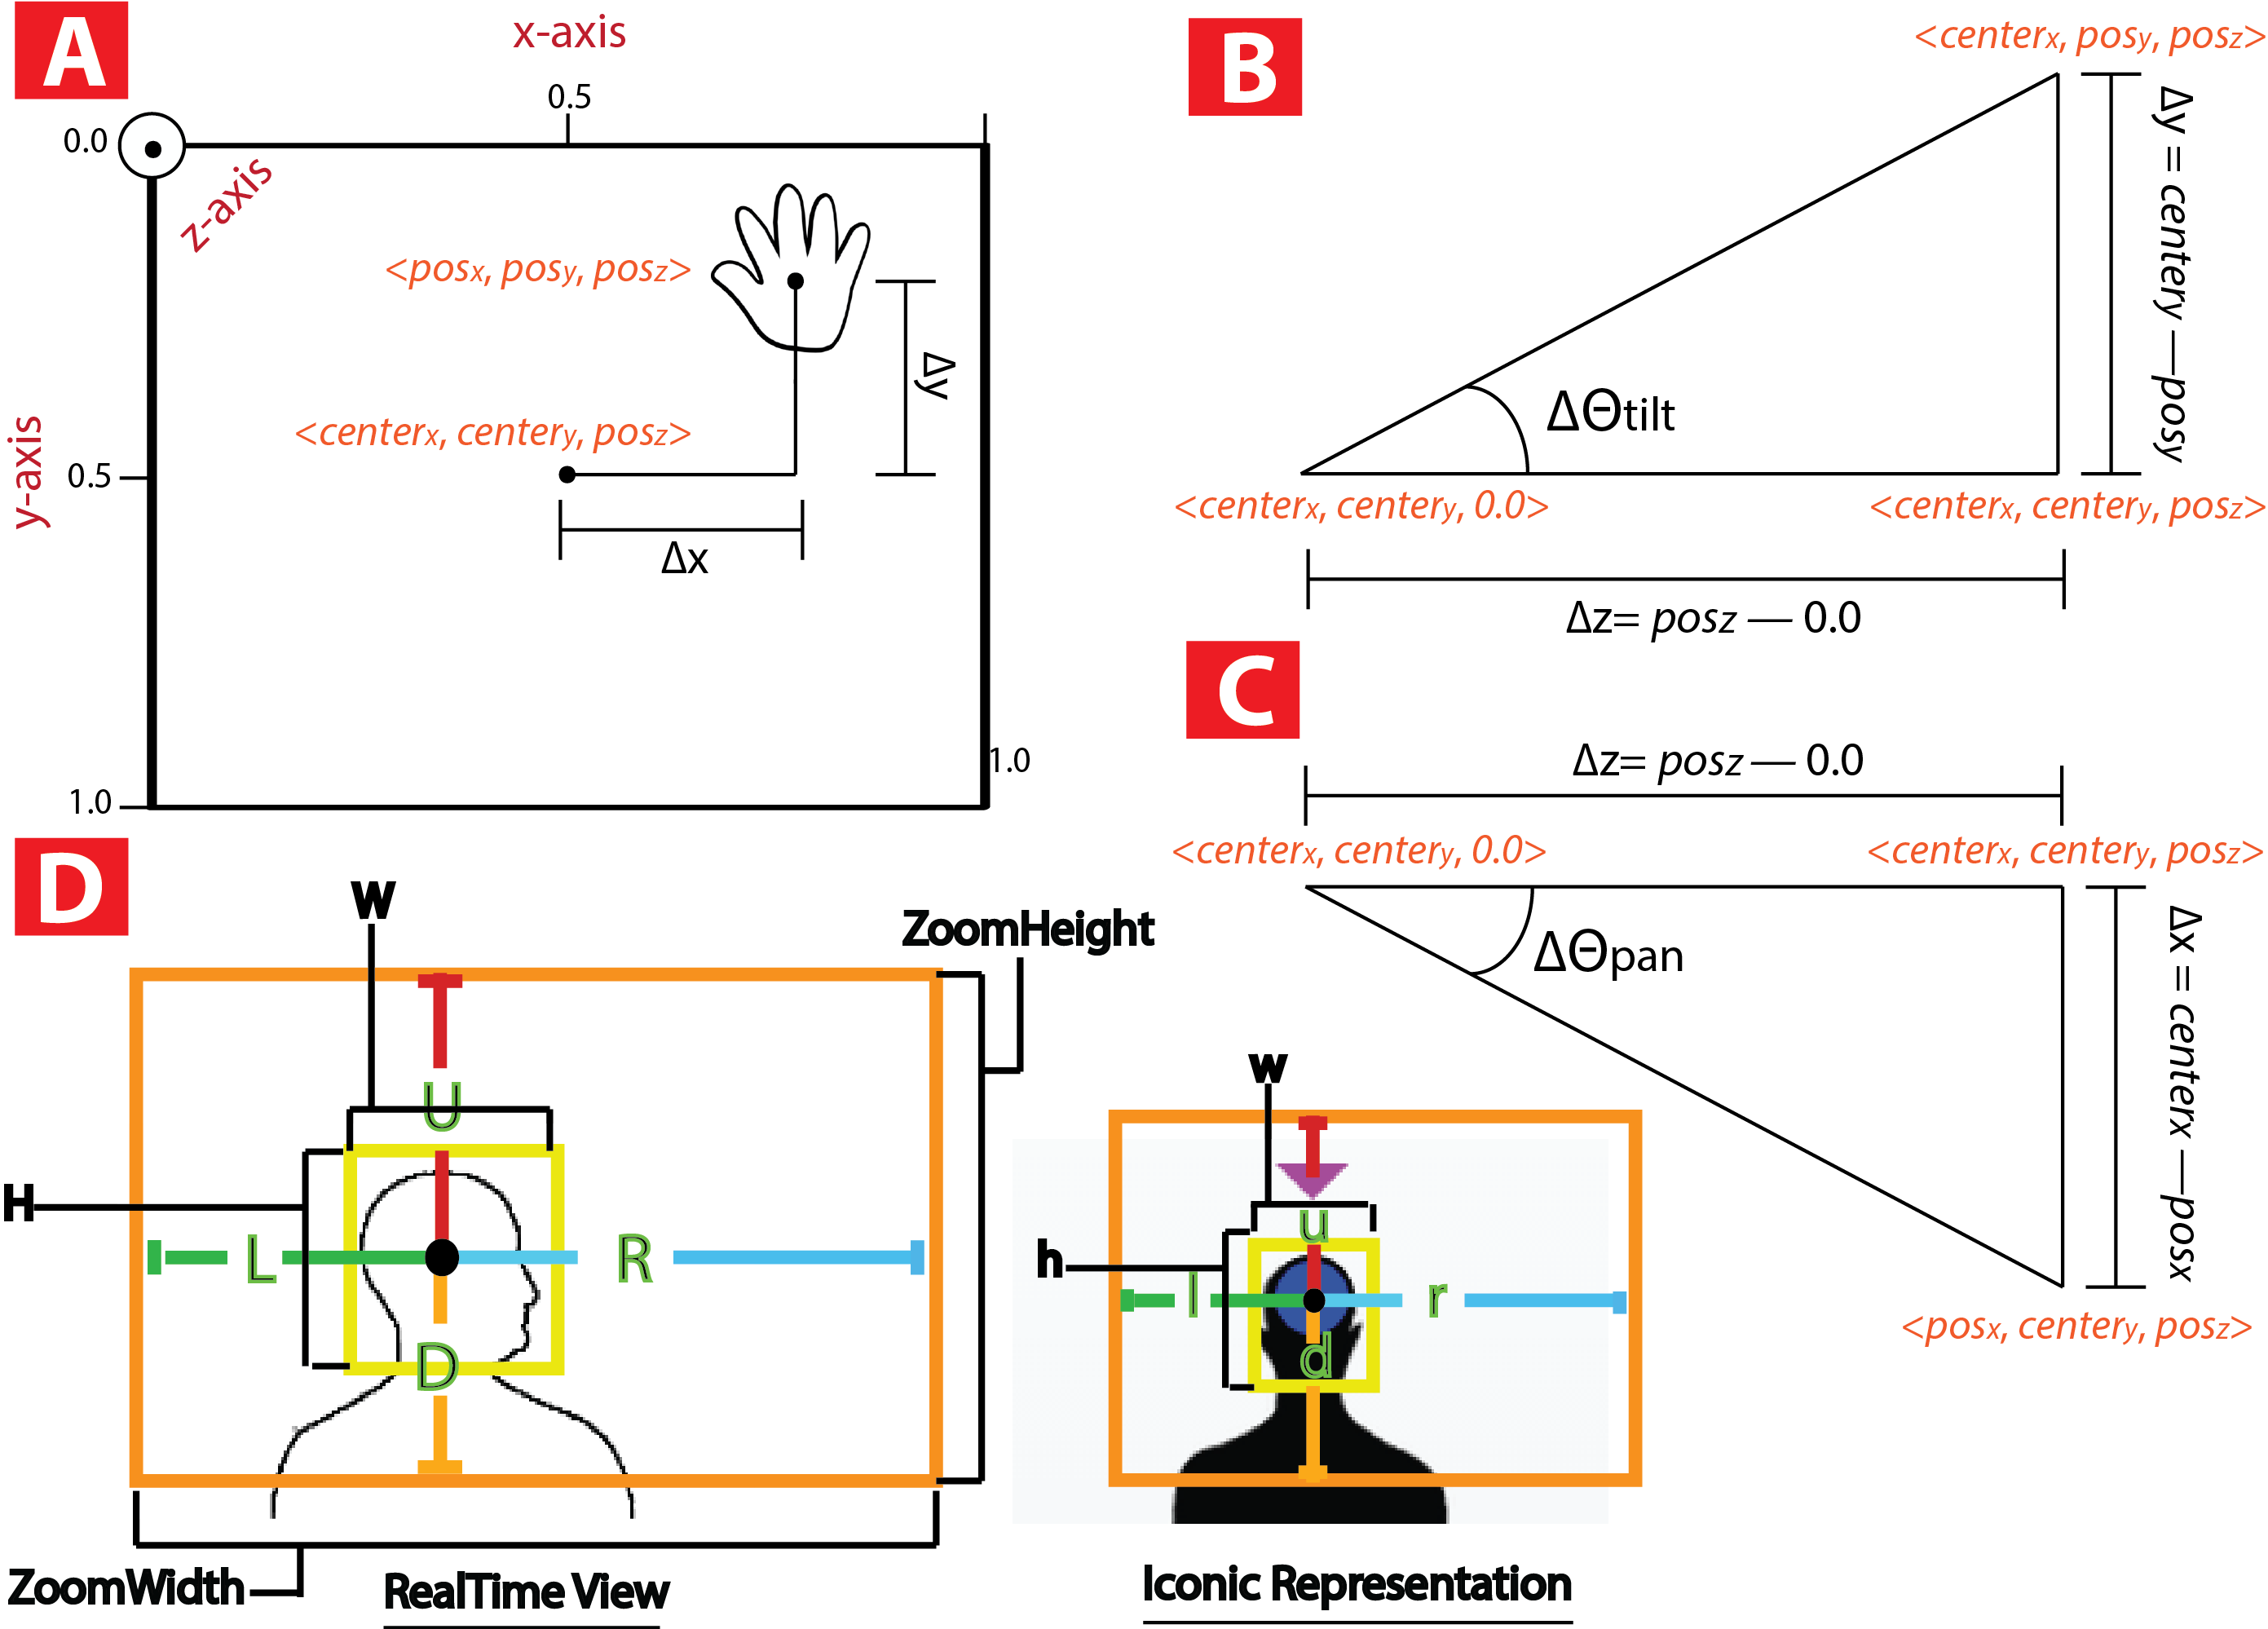
\includegraphics[width=0.7\columnwidth]{\kinectograph/fig/MathFinal}
\caption{Kinectograph tracks the position of the target (A) and computes the tilt (B) and the pan (C) angles in order to center the target. It digitally zooms the camera view based on user specified region on the Tablet UI (D).}
\label{fig:math}
\end{figure}

\subsubsection{Digital Tracking and Zooming}
% \bh{The Kinect has fixed field of view so we perform digital zoom. This is valuable in demonstration videos to direct the viewer's attention. For higher resolution zooming, future hardware embodiments could either employ a camera with programmable region-of-interest on the sensor, or a camera with a programmatically controllable zoom lens.}

% \bh{Describe how you zoom in initially; when you decide to zoom out, and why you made these decisions.}
Users may find it important not only to center a joint in the view but also magnify it, such as zooming into the hand during a demonstration showing how to stir the ingredients.
%
Thus, Kinectograph allows users to digitally zoom into a specific area with one or more joints. Our algorithm attempts to keep the joint(s) in the same relative position as it was in its initial zoomed in view. This feature works independently of the physical tracking and thus does not require physically controlling the motors or camera.
%
Kinectograph allows the the user to draw a box on the figure in the UI around the joint she wishes to digitally track. The initial dimensions and positions of that translated zoomed region on the live video stream is determined as follows (Figure~\ref{fig:math}D), where:

$ZoomWidth= R + L = \frac{W}{2}*\frac{l}{\frac{w}{2}} + \frac{W}{2}*\frac{r}{\frac{w}{2}}$ \\
$ZoomHeight= U + D = \frac{H}{2}*\frac{u}{\frac{h}{2}}+ \frac{H}{2}*\frac{d}{\frac{h}{2}}$

After the zoomed region's initial dimension has been set, the center of this region is continuously shifted using the following equations: $\Delta X = pos_{x}^{'}-pos_{x}$ and $\Delta Y = pos_{y}^{'}-pos_{y}$

% \begin{figure}[t]
% \centering
% 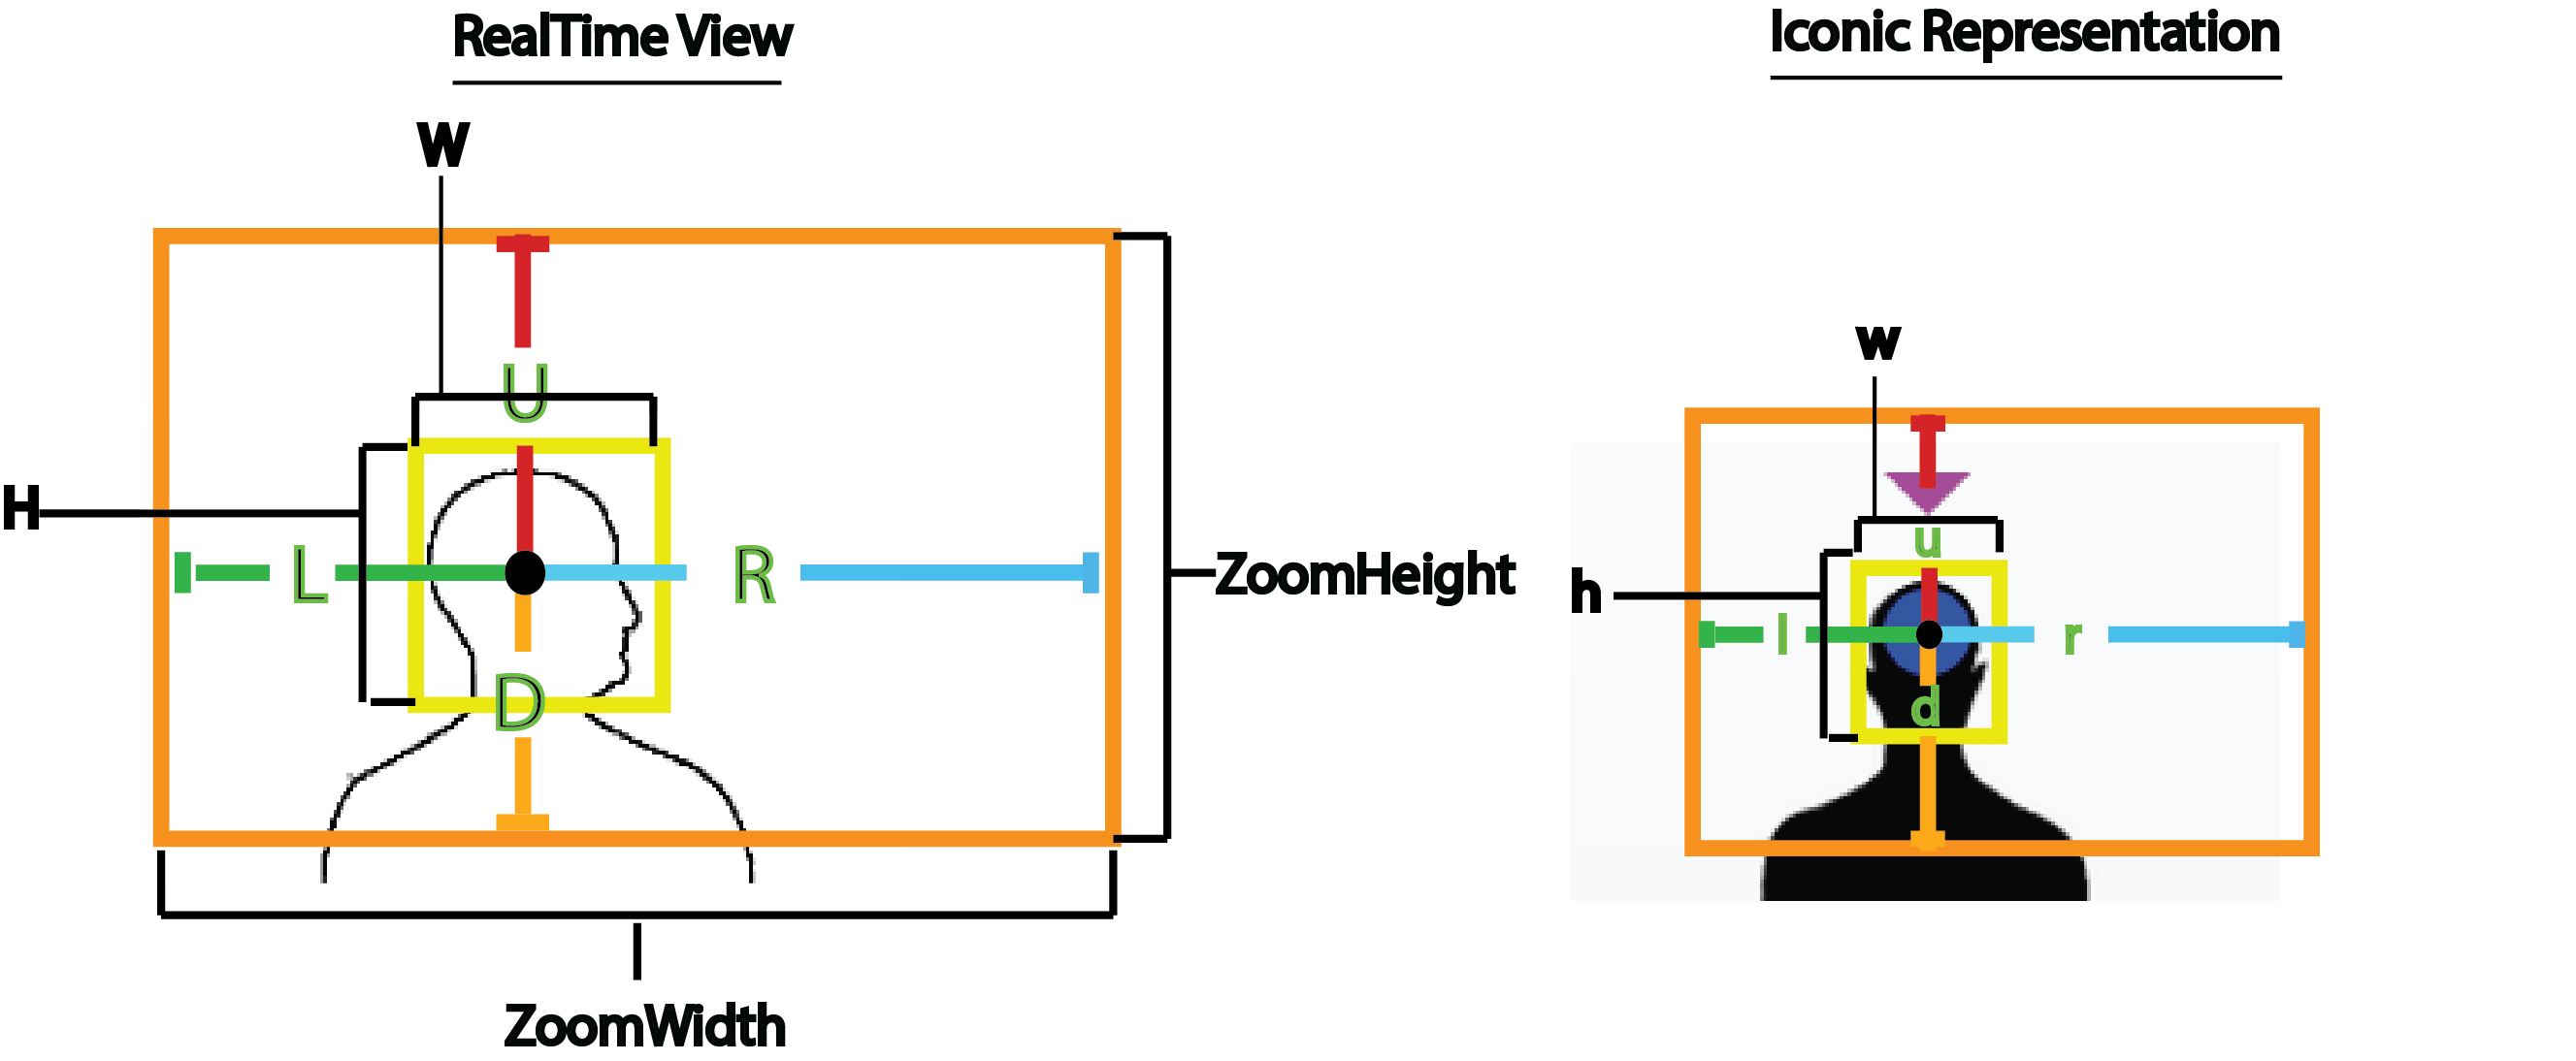
\includegraphics[width=1.0\columnwidth]{Zoom}
% \caption{Describes the the initial dimensional sizing of the zoom region}
% \label{fig:zoom}
% \end{figure}
